\begin{figure*}[h!]
\centering
\begin{adjustwidth}{-1em}{-1em}
\vspace*{-1ex}
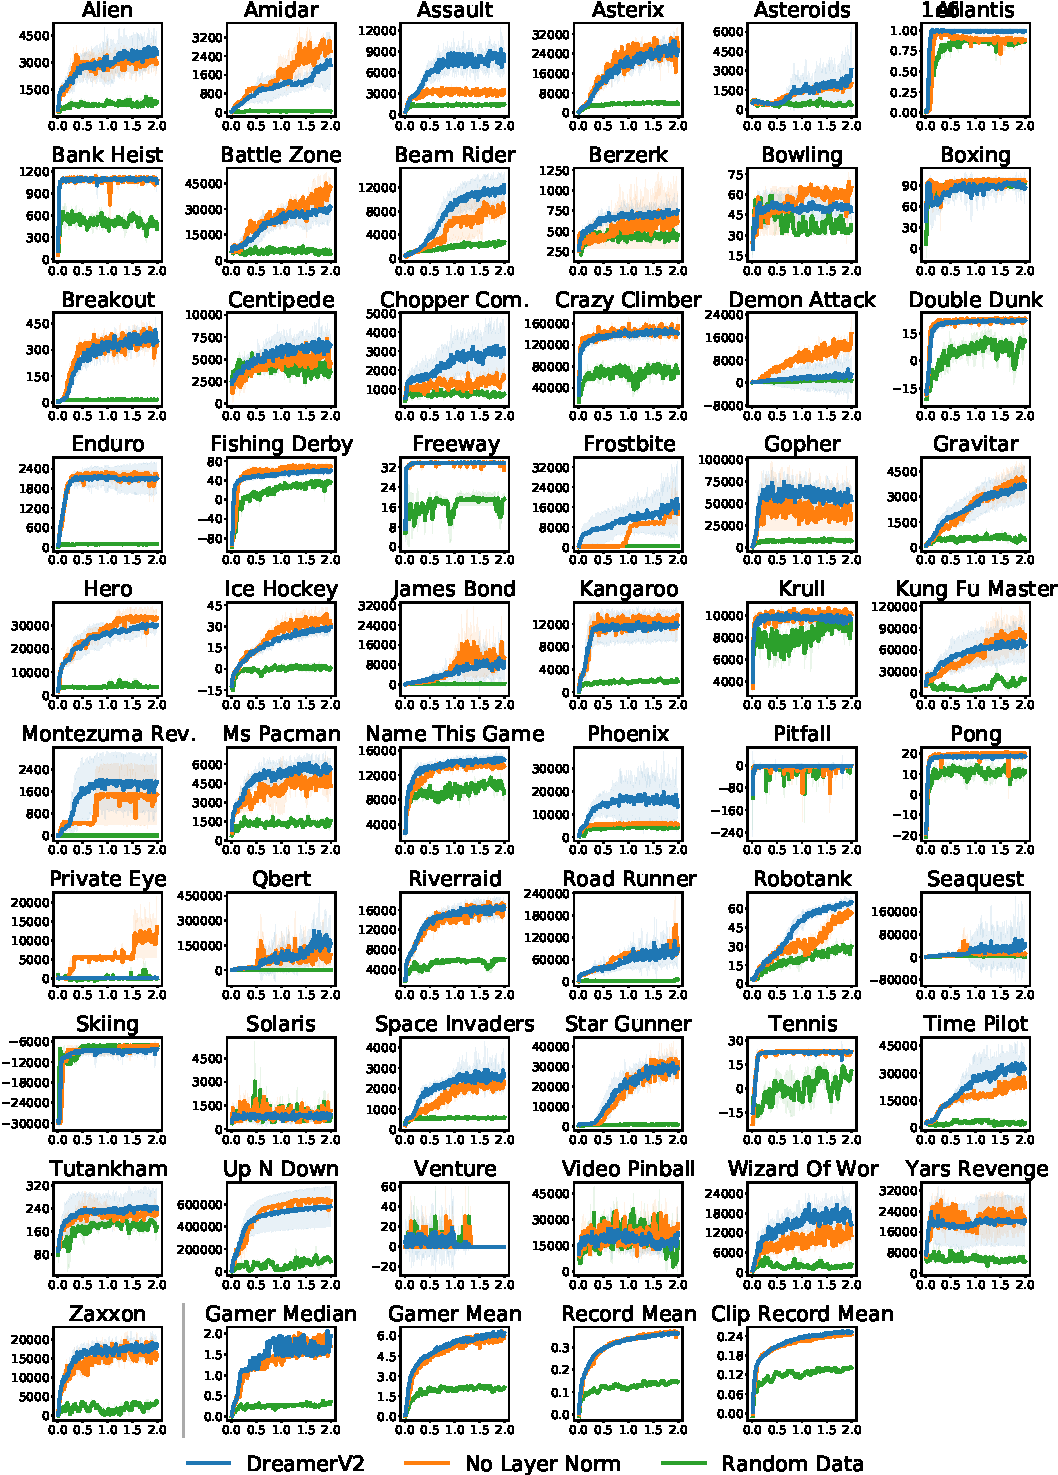
\includegraphics[width=\linewidth]{tasks-other/tasks-other}
\end{adjustwidth}
\caption{Comparison of DreamerV2 to a version without layer norm in the GRU and to training from experience collected over time by a uniform random policy. We find that the benefit of layer norm depends on the task at hand, increasing and decreasing performance on a roughly equal number of tasks. The comparison to random data collection highlights which of the tasks require non-trivial exploration, which can help guide future work on directed exploration using world models.}
\label{fig:tasks-other}
\vspace*{-2ex}
\end{figure*}
